\section{Task 3}

\setcounter{task}{1}
\begin{frame}{Task 3}{Marked Graphs}
    \begin{tasknoinc}
        Consider the following marked graph:
        \begin{figure}
            \centering
            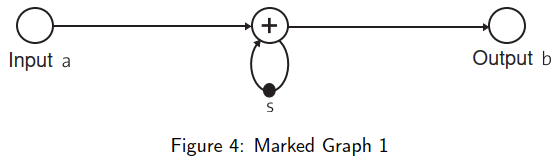
\includegraphics[scale=0.6]{figures/markedGraph.PNG}
        \end{figure}
        At the input a a sequence of numbers is read in, with a(k) representing the k-th number. Determine the outgoing sequence b(k) as function of the input values.
    \end{tasknoinc}
\end{frame}
\begin{frame}{Task 3}{Marked Graphs}
    \begin{requirementsnoinc}
        Marked graphs:
        \begin{itemize}
            \item The \alert{token} on the edges correspond to data that are stored in \alert{FIFO} queues.
            \item A node is called \alert{actor}, it is \alert{activated} if on every input edge there is at least one token.
            \item An actor can \alert{fire} if it is activated.
            \item The \alert{firing of a node} removes or consumes from each input edge a token and adds a token to each output edge. The output token corresponds to the processed data.
        \end{itemize}
    \end{requirementsnoinc}
\end{frame}
\begin{frame}{Task 3}{Marked Graphs}
    \begin{solution}
    \begin{figure}
        \centering
        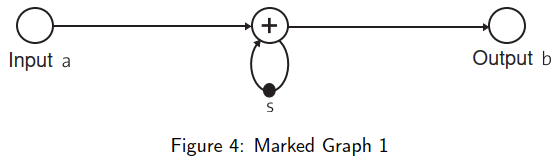
\includegraphics[scale=0.6]{figures/markedGraph.PNG}
    \end{figure}
    \begin{itemize}
        \item For $b(1)$ it is clear that $b(1) = a(1) + s$
        \item When the + actor fires, it puts $b(1)$ on both its outgoing edges, meaning $b(1)$ is propagated back onto the looping edge as well!
        \item Hence, for $b(2)$ we obtain $b(2) = a(2) + b(1)$.
        \item In general: $b(k) = a(k) + b(k-1)$
    \end{itemize}
    \end{solution}
\end{frame}
\begin{frame}{Task 3}{Marked Graphs}
    \begin{tasknoinc}
        The initial mark with the value s is replaced by n marks $s_1, ..., s_n$. Determine a recursive formula for the output sequence b(k).
    \end{tasknoinc}
\end{frame}
\begin{frame}{Task 3}{Marked Graphs}
    \begin{solutionnoinc}
        \begin{figure}
            \centering
            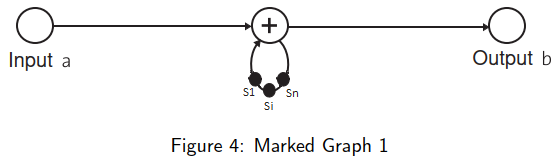
\includegraphics[scale=0.35]{figures/markedGraph2.png}
        \end{figure}
        \begin{itemize}
            \item Note that only three of the $n$ tokens are shown in the image above.
            \item Case 1: If $n = 0$ the output sequence is empty.
            \item Case 2: If $k \leq n$ we can describe the output as $b(k) = a(k) + s(k)$. Since the initial tokens on the looping edge will not run out.
            \item Case 3: If $k > n$ we can describe the output as $b(k) = a(k) + b(k-n)$. Since the initial tokens on the looping edge will run out. With each computation, we enqueue $b(0), b(1)...$ to the looping edge, supplying the computation after all $s_i$, $1 \leq i \leq n$ were consumed.
        \end{itemize}
    \end{solutionnoinc}
\end{frame}